\chapter{Methodology} \label{CH:method}

Throughout the course of this research various schemes were attempted, often as a reaction to the problems arising in simulation dynamics. Because the code has undergone so many modifications, it is not reasonable to provide results from every attempt. Instead, this chapter aims to provide the reader with a generalized overview of the various methods that were attempted and provide insight into the logic behind the decisions that were made. It is be helpful to be aware that there are three main components to the method presented in this work: fine grid height functions, fine grid velocity establishment, and fine grid flux integration. Each of these constituent pieces are complex and affect the overall effectiveness of the method. While the following sections describe these as separate pieces, it is important to recognize that development occurred concurrently and modification to these different approaches may have occurred out of the order that is presented. For ease of explanation, separate sections will be devoted to the three portions and will attempt to provide a thorough discussion of the strengths and shortcomings of each.

\section{Problem Statement}
When a dual grid is used, the standard height function method fails to capture the dynamics occurring on the fine grid. Left unmitigated, these dynamics can lead to fine grid interfacial perturbations (small discontinuities in interface structures). These perturbations can grow uncontrollably and result in non-physical dynamics materializing in simulations. An example of this uncontrolled growth resulting in non-physical dynamics can be seen in Figure~\ref{bad2}. The focus of this research is to develop an extension of the standard height function to include information from the Rudman dual mesh. The proposed  fine grid method retains the benefit of consistent mass and momentum transport while also providing accurate curvature calculations that result in interface transport that avoids non-physical dynamics. 
\begin{figure}[htbp]
	\centering
	\includegraphics[width=0.3\textwidth]{figs/bad.png}
	\caption{Standard height function method interface breakup.}
	\label{bad2} 
\end{figure} 

\subsection{Solution Overview}
When considering how to inform the coarse grid from the finer mesh, a natural direction is to adopt a height function method directly onto the fine grid. Implementing a height function is straightforward as previously described and, the same coarse grid curvature stencil should result in a more accurate curvature estimation as there is more information available from the fine grid. Figure \ref{fig:fgHFM} gives an example of what this could look like. Notice that while the stencil that the curvature is computed over remains the same as in Figure~\ref{fig:hts}, there are now twice as many heights since information is pulled from columns built from fine grid cells. However, this implementation alone does not provide a satisfactory result. Additionally, a fine grid velocity correction is added to reduced interfacial perturbations. These fine grid velocities are then incorporated into the cell flux using streak tubes. 
\begin{figure}[h]
	\centering
	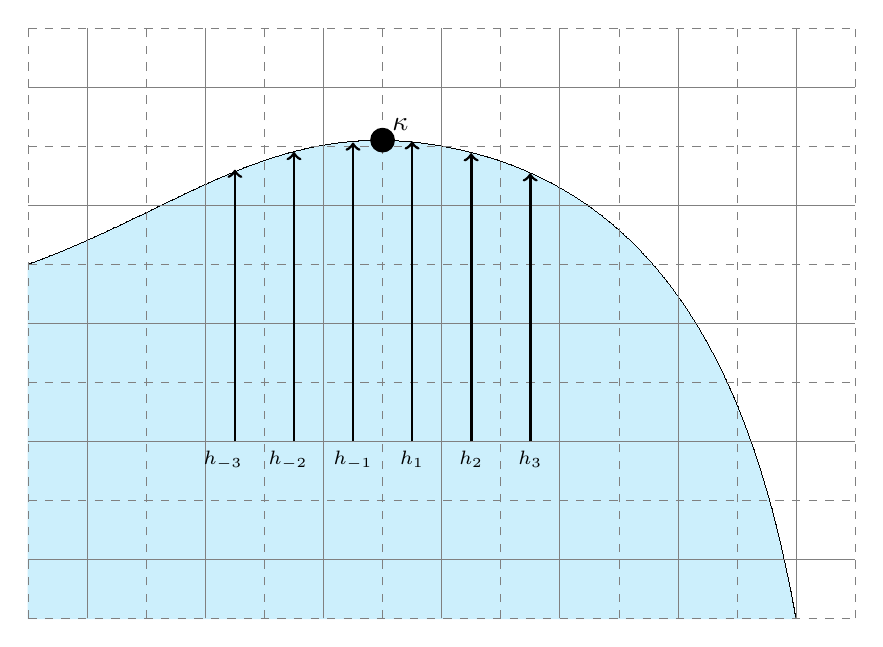
\begin{tikzpicture}[scale=1.5]
	% Liquid
	\draw [line width=0,fill=cyan!20] (0.5,3.5) to[out=20,in=170] (4,4.5) to[out=-10,in=100] (7.0,0.5);
	\draw [cyan!20,fill=cyan!20] (0.5,3.5) -- (7.0,0.5) -- (0.5,0.5) -- cycle;
	% \node [] at (0.25,3.5) {$\Gamma$};
	% Mesh
	\draw [step=1.0, help lines] (0.5 , 0.5) grid (7.5,5.5);
	\draw [dashed,step=0.5, help lines] (0.5 ,0.5) grid (7.5,5.5);
	% kappa 1
	\draw [fill] (3.5,4.55) circle [radius=0.1];
	\node [above right] at (3.5,4.55) {$\kappa$};
	\draw [arrows=->,line width=1.0] (2.25,2) -- (2.25,4.3);  \node [below] at (2.15,2.0) {\scriptsize $h_{\text{-}3}$};
	\draw [arrows=->,line width=1.0] (2.75,2) -- (2.75,4.45);\node [below] at (2.70,2.0) {\scriptsize $h_{\text{-}2}$};
	\draw [arrows=->,line width=1.0] (3.25,2) -- (3.25,4.53);\node [below] at (3.25,2.0) {\scriptsize $h_{\text{-}1}$};
	\draw [arrows=->,line width=1.0] (3.75,2) -- (3.75,4.54);\node [below] at (3.75,2.0) {\scriptsize $h_{1}$};
	\draw [arrows=->,line width=1.0] (4.25,2) -- (4.25,4.44);\node [below] at (4.25,2.0) {\scriptsize $h_{2}$};
	\draw [arrows=->,line width=1.0] (4.75,2) -- (4.75,4.27);\node [below] at (4.75,2.0) {\scriptsize $h_{3}$};	    
	\end{tikzpicture}
	\caption{Fine grid height function with the same three coarse grid cell stencil as in Fig.~\ref{fig:hts}. Here, dashed lines show fine grid boundaries while solid lines indicate coarse grid boundaries.}
	\label{fig:fgHFM}
\end{figure}

\subsection{Method Evaluation - Test Cases}
To further quantify the problem that is occurring, baseline test cases which highlight the shortcomings of current methods are necessary. To this end, the height function method functionality is evaluated by calculating the curvature of an exactly defined VOF field. The curvature of a circle for example, is exactly equal to the reciprocal of the radius as seen in Figure~\ref{fig:curv}. A static circle is represented by an exact VOF field and the method computes the curvature. Results are compared against an analytic solution. 

Additionally, an oscillating two-dimensional droplet is used to assess the height function method and the proposed solution methods in a dynamic environment. This test case was chosen as it is considered a standard benchmark problem for testing the accurate prediction of multiphase flow behavior~\cite{Salih2002}. Additionally, for the height function method, the oscillating droplet offers an extensive testing of interface orientations which is important for measuring the robustness of the method. The interface is initialized as an ellipse. Surface tension drives the droplet's semi-major axis to fluctuate between alignment with the $x$ and $y$ axes as seen in Figures~\ref{fig:Odrop1}~-~\ref{fig:Odrop3}. 
\begin{figure}[htbp]
	\centering
	\begin{subfigure}{.3\textwidth}
		\centering
		\includegraphics[width=1.0\linewidth]{figs/Odrop1}
		\caption{An ellipse is initialized in the domain.}
		\label{fig:Odrop1}
	\end{subfigure}%
\hfill
	\begin{subfigure}{0.3\textwidth}
		\centering
		\includegraphics[width=1.0\linewidth]{figs/Odrop2}
		\caption{Surface tension begins driving motion.}
		\label{fig:Odrop2}
	\end{subfigure}
\hfill
\begin{subfigure}{0.3\textwidth}
	\centering
	\includegraphics[width=1.0\linewidth]{figs/Odrop3}
	\caption{Droplet extends and oscillation continues.}
	\label{fig:Odrop3}
\end{subfigure}
\caption{An oscillating droplet test case.}
\end{figure}
The period of oscillation $T_{e}$, is a function of surface tension coefficient ($\sigma$), density ($\rho_l$ and $\rho_g$), and equivalent circular radius($R$), where 
\begin{equation}
R = \sqrt{a^2+b^2}
\end{equation}and $a$ and $b$ are the semi-major and semi-minor axes respectively. The oscillation period can be computed analytically as~\cite{Rayleigh}
\begin{equation}
T_{e} = 2 \pi \sqrt{\frac{(\rho_{l}+\rho_{g})R^3}{6\sigma}}.
\label{period}
\end{equation}

Simulation parameters include a density ratio of 1000, viscosity in both the liquid and gas phases are zero, and no walls are present in the computational domain. An ellipse with a center at the origin and a major axis parallel to the x-axis can be described as 
\begin{equation}
\frac{x^2}{a^2} + \frac{y^2}{b^2} =1.
\end{equation}  
Within the test case, $a$ and $b$ are explicitly defined. A semi-major radius of $a=0.24$ and a semi-minor axes radius of $b=0.20$ define the initial displacement of the droplet. The total domain length is set to 1.0. These parameters are chosen as they align with the analytic solution assumptions made. For the initial baseline, a mesh of 64x64 grid cells make up the domain. The mesh size was chosen specifically to address a concern for having a sufficient number of grid cells across the diameter of the droplet. A sufficient number of grid cells across a diameter can be considered as any minimum number of cells which provide well defined heights to the height function.

 Figure~\ref{fig:acesKE} shows kinetic energy conservation through the progression of the oscillating droplet simulation. Simulation success is quantified by normal periods of oscillation and diminishing kinetic energy with time. In an ideal case, no diminishment of kinetic energy would occur as the case is set up such that no energy can be lost to viscosity or boundary conditions. However, due to numerical dissipation, this loss is often observed. Close adherence to the solution in Figure~\ref{fig:acesKE} can be used as a measure of success with methods from here forward.
\begin{figure}[htpb]
	\centering
	\includegraphics[width=0.5\textwidth]{figs/ACES_KEplot.png}
	\caption{For the oscillating droplet test case, capturing kinetic energy over time is a way to discern whether the model is progressing as desired. Regular periods and linearly decreasing kinetic energy represent a favorable result. Simulation using ACES Method~\cite{Owkes2018}}
	\label{fig:acesKE}
\end{figure}
Alternatively, Figure \ref{fig:stdKE} shows the result of the same test case ran with a standard, coarse grid, curvature estimation scheme. The uncontrolled growth in kinetic energy seen in the standard method is a result of the aforementioned interfacial perturbations. The curvature estimation error and resulting non-physical dynamics are the motivation for this research. 
\begin{figure}[htpb]
	\centering
	\includegraphics[width=0.5\textwidth]{figs/stdHt_KEplot.png}
	\caption{Kinetic Energy with Time - Standard Height Function Method(Solid) vs ACES method(Dashed)}
	\label{fig:stdKE}
\end{figure}
 
 \section{Fine Grid Height Function Methods}
 As previously stated, this section will provide an outline of several methodologies used to compute a fine grid curvature calculation. The goal of using a fine grid height function is to utilize information gained from our now twice as fine mesh (from Rudman's method) to predict a more accurate estimate of our curvature value.
 \subsection{Fifth Order Method}
\begin{figure}[htbp]
	\centering
	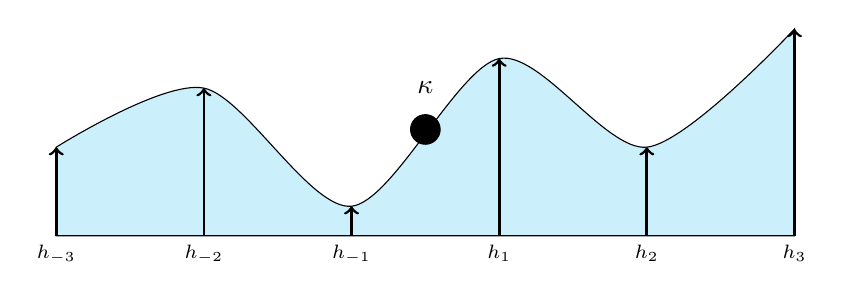
\begin{tikzpicture}[scale=3.75]
	% Heights
	\draw [black, fill=cyan!20] plot [smooth ] coordinates {(0.25,0.3)(0.75,0.5)(1.25,0.1)(1.75,0.6)(2.25,0.3)(2.75,0.7)} -- (2.75,0) -- (0.25,0) -- cycle;
	\draw [fill] (1.5,0.36) circle [radius=0.05];
	\node [above ] at (1.5,0.45) {$\kappa$};
	\draw [arrows=->,line width=1.0] (0.25,0) -- (0.25,0.3);\node [below] at (0.25,0) {\scriptsize $h_{-3}$};
	\draw [arrows=->,line width=1.0] (0.75,0) -- (0.75,0.5);\node [below] at (0.75,0) {\scriptsize $h_{-2}$};
	\draw [arrows=->,line width=1.0] (1.25,0) -- (1.25,0.1);\node [below] at (1.25,0) {\scriptsize $h_{-1}$};
	\draw [arrows=->,line width=1.0] (1.75,0) -- (1.75,0.6);\node [below] at (1.75,0) {\scriptsize $h_{1}$};
	\draw [arrows=->,line width=1.0] (2.25,0) -- (2.25,0.3);\node [below] at (2.25,0) {\scriptsize $h_{2}$};
	\draw [arrows=->,line width=1.0] (2.75,0) -- (2.75,0.7);\node [below] at (2.75,0) {\scriptsize $h_{3}$};
	\end{tikzpicture}
	\caption{Proposed $5^{th}$ order fit of heights using columns built from fine grid cells. }
	\label{fig:5hts}
\end{figure}

As seen in Figure \ref{fig:fgHFM}, there are now six columns over which information is being provided. With this information, it is possible to derive fifth order approximations for the first and second derivatives needed for the curvature calculation. Figure~\ref{fig:5hts} gives an approximate representation of what a fit might look like for a given point. A general formula for deriving a finite difference approximation given a set of points is given as 
\begin{equation}
h'_j + \sum_{k=-3}^{3} a_k h_{j+k} = O(?).
\label{eqn:gen}
\end{equation}
\begin{figure}[htbp]
	\centering
	\includegraphics[width=0.5\linewidth]{figs/findiff.png}
	\caption{Given a set of three points along a continuous function, it is possible to calculate a second order finite difference operator.}
	\label{fig:findiff}
\end{figure}
%\begin{equation}
%\frac{dh}{dx} = a_{-3}h_{-3} +a_{-2}h_{-2} + a_{-1}h_{-1} + a_{+1}h_{+1} + a_{+2}h_{+2} + a_{+3}h_{+3} .
%\label{eqn:poly}
%\end{equation}
Assume we are interested in computing the most accurate finite difference operator for a given set of points which pass through a continuous function as seen in Figure~\ref{fig:findiff}. We have three points with a span of $\Delta x$ between each point. Finding an approximation for the first derivative is achieved by writing the Taylor series for each of the points
\begin{equation}
H_{j-1} = H_j - \Delta x H'_j + \frac{\Delta x^2}{2} H''_j- \frac{\Delta x^3}{6} H'''_j 
\label{eqn:tay1}
\end{equation}
\begin{equation}
H_{j+1} = H_j - \Delta x H'_j + \frac{\Delta x^2}{2} H''_j- \frac{\Delta x^3}{6} H'''_j
\label{eqn:tay2}
\end{equation}
and taking their difference which results in 
\begin{equation}
H_{j-1} - H_{j+1} = 2\Delta x H'_j - \frac{\Delta x^3}{3} H'''_j.
\label{eqn:diff}
\end{equation}
Using this difference, we find the approximation for the first derivative to be 
\begin{equation}
H'_j = \frac{H_{j+1} - H_{j-1}}{2\Delta x} + \frac{\Delta x^2}{3} H'''_j.
\label{eqn:poly}
\end{equation}

\begin{figure}[htbp]
	\centering
	\includegraphics[width=0.75\linewidth]{figs/properhts.png}
	\caption{An appropriate fine grid height function requires integral values of heights as opposed to point-wise values.}
	\label{fig:int}
\end{figure}
This same technique can be extrapolated to a fifth order approximation given the six points of interest we have as illustrated by Figure~\ref{fig:5hts}. However, this provides an incomplete assessment of the derivatives which are needed for our curvature estimation. While the above method provides the Taylor series approximation needed for a point-wise fitting function, column heights used in the height function method require integral quantities of the Taylor series. This is because VOF values are also integral quantities, not point-wise quantities. This nuanced distinction is illustrated in Figure~\ref{fig:int}. For this adjustment, the same basic principal applies. A Taylor series expansion is performed to find function values over which to integrate ($H(x)$). Heights ($h_i$) are determined by integrating values of $H_x$ over the width of the subcell as \begin{equation}
h_j = \frac{1}{\Delta x}\int^{x_{j+\frac{1}{2}}}_{x_{j-\frac{1}{2}}} H(x)dx,
\label{eqn:int}
\end{equation} 
where $H_x$ is approximated using a Taylor series as 
\begin{equation}
H(x) = H(x_j) + (x-x_j)H'(x_j) + \frac{ (x-x_j)^2}{2} H''(x_j) + ... .
\end{equation}
Evaluating the integral provides us with an approximation for our height as 
\begin{equation}
h_j = H(x_j) + \frac{ \Delta x }{2} H'(x_j) + ...
\end{equation}
 applied over the interval from ${x_{j-\frac{1}{2}}}$ to ${x_{j-\frac{1}{2}}}$.With heights determined, coefficients needed for derivative approximation are found. Code which details the determination of coefficients can be seen in the Appendix. Figures~\ref{fig:wts1}~\&~\ref{fig:wts2} show the method solution for a first and second derivative evaluated against a forth and fifth order error and provide evidence that the method provides fifth order accuracy for a first derivative approximation. However, for a second derivative approximation, we find that the method holds to forth order accuracy.  Upon further investigation, we found that the Taylor's series for a second derivative results in a error term on the order of $\frac{\Delta x^6}{\Delta x^2}$, which results in a forth order error approximation ($\Delta x^4$). Therefore, this limits the overall curvature estimation to forth order accuracy. However, we were still pleased with this improvement over a standard height function which is second order accurate.
 \begin{figure}[htbp]
 	\centering
 	\begin{minipage}{.45\textwidth}
 		\centering
 		\includegraphics[width=1.0\linewidth]{figs/WeightsDer2.png}
 		\caption{Improved $5^{th}$ order method approximating a first derivative. The method still holds approximately $5^{th}$ order accuracy.}
 		\label{fig:wts1}
 	\end{minipage}%
 	\hfill
 	\begin{minipage}{0.45\textwidth}
 		\centering
 		\includegraphics[width=1.0\linewidth]{figs/WeightsDer3.png}
 		\caption{Improved $5^{th}$ order method approximating a second derivative. The method holds approximately $4^{th}$ order accuracy.}
 		\label{fig:wts2}
 	\end{minipage}
 \end{figure}
 With the successful implementation, the method was again tested using the oscillating droplet test case. Here, instead of the dissipation of kinetic energy we saw behavior similar to that of the standard height function method. The scheme was stable initially and then kinetic energy grew uncontrollably until eventual simulation failure.
%Here, $a_k$ are the coefficients associated with the linear Taylor series which need to be solved for~\cite{moin}. For the six heights given by our fine grid stencil, Table \ref{tab:findiff} shows how the linear equations can be formed to find the first derivative.
%\begin{table}[tbp]
%	\centering
%	\caption{Taylor Series for Fifth Order First Derivative }
%		\begin{tabular}{c|c|c|c|c|c|c|c} % <-- Alignments: 1st column left, 2nd middle and 3rd right, with vertical lines in between
%			\textbf{}          &\textbf{$f$} & \textbf{$f'$}            & \textbf{$f''$}                                 & \textbf{$f'''$}                                 & \textbf{$f^{iv}$}                             & \textbf{$f^{v}$}                                \\
%			\hline
%			$f'$                                     & 0                                     & 1                                                       &                                                    0       &                                                              0&                                                      0&                                                                     0&\\
%			$a_{\text{-}3}f_{\text{-}3}$& $\frac{a_{\text{-}3}}{0!}$ &$a_{\text{-}3}\frac{(\text{-}3h)}{1!}$ &$a_{\text{-}3}\frac{(\text{-}3h)^2}{2!}$  &$a_{\text{-}3}\frac{(\text{-}3h)^3}{3!}$   &$a_{\text{-}3}\frac{(\text{-}3h)^4}{4!}$    &$a_{\text{-}3}\frac{(\text{-}3h)^5}{5!}$   &\\ 
%			$a_{\text{-}2}f_{\text{-}2}$& $\frac{a_{\text{-}2}}{0!}$ &$a_{\text{-}2}\frac{(\text{-}2h)}{1!}$ &$a_{\text{-}2}\frac{(\text{-}2h)^2}{2!}$  &$a_{\text{-}2}\frac{(\text{-}2h)^3}{3!}$   &$a_{\text{-}2}\frac{(\text{-}2h)^4}{4!}$    &$a_{\text{-}2}\frac{(\text{-}2h)^5}{5!}$   &\\
%			$a_{\text{-}1}f_{\text{-}1}$& $\frac{a_{\text{-}1}}{0!}$ &$a_{\text{-}1}\frac{(\text{-}h)}{1!}$   &$a_{\text{-}1}\frac{(\text{-}h)^2}{2!}$    &$a_{\text{-}1}\frac{(\text{-}h  )^3}{3!}$   &$a_{\text{-}1}\frac{(\text{-}h )^4}{4!}$     &$a_{\text{-}1}\frac{(\text{-}h )^5}{5!}$    &\\
%			$a_{+1}f_{+1}$                   & $\frac{a_{+1}}{0!}$           &$a_{+1}\frac{(h)}{1!}$                         &$a_{+1}\frac{(h)^2}{2!}$                         &$a_{+1}\frac{(\frac{h}{2})^3 }{3!}$           &$a_{+1}\frac{(\frac{h}{2})         ^4}{4!}$     &$a_{+1}\frac{(\frac{h}{2})^5}{5!}$             &\\
%			$a_{+2}f_{+2}$                   & $\frac{a_{+2}}{0!}$           &$a_{+2}\frac{(2h)}{1!}$                       &$a_{+2}\frac{(2h)^2}{2!}$                       &$a_{+2}\frac{(\frac{2h}{2})^3}{3!}$          &$a_{+2}\frac{(\frac{2h}{2})       ^4}{4!}$     &$a_{+2}\frac{(\frac{2h}{2})^5}{5!}$           &\\
%			$a_{+3}f_{+3}$                  & $\frac{a_{+3}}{0!}$            &$a_{+3}\frac{(3h)}{1!}$                       &$a_{+3}\frac{(3h)^2}{2!}$                       &$a_{+3}\frac{(\frac{3h}{2})^3}{3!}$          &$a_{+3}\frac{(\frac{3h}{2})       ^4}{4!}$     &$a_{+3}\frac{(\frac{3h}{2})^5}{5!}$           &\\
%		\end{tabular}
%		\label{tab:findiff}
%\end{table}
%Traditionally, from the columns in Table~\ref{tab:findiff}, six equations can be used to solve for the six unknown variables. With these coefficients, approximations can be derived for a fitting function. The first iteration of the $5^{th}$ order height function used the above method to determine a polynomial with which to pass our heights through. Figure~\ref{fig:1stDer} shows the solution of the resulting fifth order finite difference first derivative used to approximate a solution of $e^x$ plotted against an analytic solution. Figure \ref{fig:1stErr} provide quantifying evidence that the method holds fifth order accuracy to machine precision.  Figures~\ref{fig:2ndDer} and~\ref{fig:2ndErr} show similar behavior and similar stability for the solution of the second derivative.
%\begin{figure}[htbp]
%	\centering
%	\begin{minipage}{.45\textwidth}
%		\centering
%		\includegraphics[width=1.0\linewidth]{figs/1stDer.png}
%		\caption{Proposed $5^{th}$ order method calculating values of $e^x$ plotted against analytic solution.}
%		\label{fig:1stDer}
%	\end{minipage}%
%\hfill
%	\begin{minipage}{0.45\textwidth}
%		\centering
%		\includegraphics[width=1.0\linewidth]{figs/1stErr.png}
%		\caption{Proposed $5^{th}$ order method approximating first derivative. Method holds $5^{th}$ order accuracy to machine precision.}
%		\label{fig:1stErr}
%	\end{minipage}
%\end{figure}
%\begin{figure}[htbp]
%	\centering
%	\begin{minipage}{.45\textwidth}
%		\centering
%		\includegraphics[width=1.0\linewidth]{figs/2ndDer.png}
%		\caption{Proposed $5^{th}$ order method calculating values of $e^x$ plotted against analytic solution.}
%		\label{fig:2ndDer}
%	\end{minipage}%
%\hfill
%	\begin{minipage}{0.45\textwidth}
%		\centering
%		\includegraphics[width=1.0\linewidth]{figs/2ndErr.png}
%		\caption{Proposed $5^{th}$ order method approximating second derivative. Method holds $5^{th}$ order accuracy to machine precision.}
%		\label{fig:2ndErr}
%	\end{minipage}
%\end{figure}
%
%The simplest test case for testing a curvature scheme is to compute the curvature of an exact VOF field. We establish a simple case where a circle is given a radius of 0.2. Initial testing of this method provided accurate representation of the exact VOF field but struggled to effectively run the oscillating droplet simulation. Subsequent investigation determined that this approximation of the $5^{th}$ order method was not sufficient for application of the height function. While the above method provides the Taylor series approximation needed for a point-wise fitting function, column heights used in the height function method require integral quantities of the Taylor series. This is because VOF values are also integral quantities, not linear quantities. For this adjustment, the same basic principal applies. A Taylor series expansion is performed to find function values over which to integrate ($h_x$). Heights ($H_i$) are determined by integrating values of $h_x$ over the area of the subcell as seen in Eqn.~\ref{eqn:int}. With heights determined, coefficients needed for derivative approximation are found using a constrained least squares approach which enforces second order accuracy. Derivatives are approximated using the heights and coefficients. Figure~\ref{fig:int} provides an approximate visualization of the scheme as it differs from the representation in Figures~\ref{fig:fgHFM}~\&~\ref{fig:5hts}.

%\begin{figure}[htbp]
%	\centering
%%	\begin{tikzpicture}[scale=1.5]
%%	% Liquid
%%	\draw [line width=0,fill=cyan!20] (0,3) to[out=-15,in=160] (2.5,2.5) to[out=-20,in=100] (5.0,0);
%%	\draw [cyan!20,fill=cyan!20] (0,3) -- (5.0,0) -- (0,0) -- cycle;
%%	% \node [] at (0.25,3.5) {$\Gamma$};
%%	% Mesh
%%	\draw [step=1.0, help lines] (0 , 0) grid (5,4);
%%	\draw [dashed,step=0.5, help lines] (0 ,0) grid (5,4);
%%	% kappa 1
%%	\draw [fill] (2.5,2.5) circle [radius=0.1];
%%	\node [above right] at (2.5,2.5) {$\kappa$};
%%	\draw [black!60,arrows=->,line width=1.0] (1.25,0) -- (1.25,2.77);  %\node [below] at (2.15,2.15) {\scriptsize $h_{\text{-}3}$};
%%	\draw [black!60,arrows=->,line width=1.0] (1.75,0) -- (1.75,2.7);%\node [below] at (2.70,2.15) {\scriptsize $h_{\text{-}2}$};
%%	\draw [black!60,arrows=->,line width=1.0] (2.25,0) -- (2.25,2.58);%\node [below] at (3.25,2.15) {\scriptsize $h_{\text{-}1}$};
%%	\draw [black!60,arrows=->,line width=1.0] (2.75,0) -- (2.75,2.4);%\node [below] at (3.75,2.15) {\scriptsize $h_{1}$};
%%	\draw [black!60,arrows=->,line width=1.0] (3.25,0) -- (3.25,2.2);%\node [below] at (4.25,2.15) {\scriptsize $h_{2}$};
%%	\draw [black!60,arrows=->,line width=1.0] (3.75,0) -- (3.75,1.9);%\node [below] at (4.75,2.15) {\scriptsize $h_{3}$};
%%	% Heights
%%	\draw[red,pattern=north west lines, pattern color=red] (1,0) rectangle (1.5,2.77);    
%%	\draw[red,pattern=north east lines, pattern color=red] (1.5,0) rectangle (2,2.7);
%%	\draw[red,pattern=north west lines, pattern color=red] (2,0) rectangle (2.5,2.58);
%%	\draw[red,pattern=north east lines, pattern color=red] (2.5,0) rectangle (3,2.4);
%%	\draw[red,pattern=north west lines, pattern color=red] (3,0) rectangle (3.5,2.2);
%%	\draw[red,pattern=north east lines, pattern color=red] (3.5,0) rectangle (4,1.9);	
%%	% Height labels
%%	\node [below] at (1.75,0) {\scriptsize $H_{i-1}$};
%%	\node [below] at (2.25,0) {\scriptsize $H_{i}$};
%%	\node [below] at (2.75,0) {\scriptsize $H_{i+1}$};
%%	\end{tikzpicture}
%\includegraphics[0.5\linewidth]{figs/properhts.png}
%	\caption{An appropriate fine grid height function requires integral values of heights as opposed to point-wise values.}
%	\label{fig:int}
%\end{figure}

%\noindent To force a symmetric solution, we assume 
%\begin{equation}
%a_{-1} = -a_1
%\end{equation}
%\begin{equation}
%a_{-2} = -a_2
%\end{equation}
%\begin{equation}
%a_{-3} = -a_3 .
%\end{equation}
%Solving these equations, we find that the trivial solutions exists for the first, third, and fifth columns. The remaining equations are
%\begin{equation}
%a_1 (2h)+ a_2 (4h)+ a_3 (6h) = -1
%\end{equation}
%\begin{equation}
%a_1 \frac{(h)^3}{3}     +a_2  \frac{(2h)^3}{3}    +a_3 \frac{(3h)^3}{3}     = 0
%\end{equation}
%\begin{equation}
%a_1 \frac{(h)^5}{60}     +a_2  \frac{(2h)^5}{60}    +a_3 \frac{(3h)^5}{60}     = 0.
%\end{equation}


\subsection{Second-Order Fine-Grid Height-Function Method}
 Fifth order polynomials as used here, can have large oscillations in the curvature calculation leading to the errors which were observed in the droplet test case. This error is likely due to the scheme being influenced by areas of both highly positive and highly negative curvature within the fit as a fifth order method can fluctuate as it passes through the heights. In a 2018 article, Owkes et al.~found that the scale with which curvature is computed on heavily influences the growth of interface perturbations~\cite{Owkes2018}. This article also suggested that at certain scales, a second order method was more agreeable with accurate interface dynamics than a fourth order method on the same scale~\cite{Owkes2018}. With this, we considered the possibility that a fifth order function on the fine grid scale may be over-fitting the points and reconstructing an interface with more perturbations than actually exist, essentially exacerbating our problem as opposed to alleviating it. 
\begin{figure}[htbp]
	\centering
	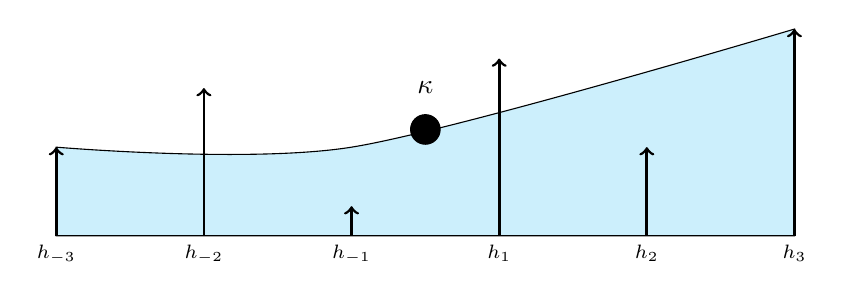
\begin{tikzpicture}[scale=3.75]
	\draw [black, fill=cyan!20] plot [smooth ] coordinates {(0.25,0.3)(1.25,0.3)(2.75,0.7)} -- (2.75,0) -- (0.25,0) -- cycle;
	\draw [fill] (1.5,0.36) circle [radius=0.05];
	\node [above ] at (1.5,0.45) {$\kappa$};
	\draw [arrows=->,line width=1.0] (0.25,0) -- (0.25,0.3);\node [below] at (0.25,0) {\scriptsize $h_{-3}$};
	\draw [arrows=->,line width=1.0] (0.75,0) -- (0.75,0.5);\node [below] at (0.75,0) {\scriptsize $h_{-2}$};
	\draw [arrows=->,line width=1.0] (1.25,0) -- (1.25,0.1);\node [below] at (1.25,0) {\scriptsize $h_{-1}$};
	\draw [arrows=->,line width=1.0] (1.75,0) -- (1.75,0.6);\node [below] at (1.75,0) {\scriptsize $h_{1}$};
	\draw [arrows=->,line width=1.0] (2.25,0) -- (2.25,0.3);\node [below] at (2.25,0) {\scriptsize $h_{2}$};
	\draw [arrows=->,line width=1.0] (2.75,0) -- (2.75,0.7);\node [below] at (2.75,0) {\scriptsize $h_{3}$};	
	\end{tikzpicture}
	\caption{The proposed $2^{nd}$ order fit still utilizes information from six fine grid heights but hopes to reduce the potential for over-fitting. }
	\label{fig:2ndhts}
\end{figure}
We decided to use the same stencil but shift to a $2^{nd}$ order polynomial. The general idea is represented in Figure~\ref{fig:2ndhts}. Calculating a $2^{nd}$ order method was done using a least squares fit of the heights.
%the same general finite difference technique as described previously but to $2^{nd}$ order accuracy. To approximate the same Taylor series to $2^{nd}$ order accuracy, a symmetry assumption was made about the coefficients. Namely that
%\begin{equation}
%	\begin{split}
%		a_{-1} = -a_1 \\
%		a_{-2} = -a_2 \\
%		a_{-3} = -a_3 
%	\end{split}
%\end{equation}
% which lead to undetermined operators that could be used as tuning parameters.
 The aim of this method was to use the same fine grid information to inform the coarse model but to smear the function to reduce unwanted perturbations. Again with mesh refinement, calculation of an exact curvature field produced encouraging results. While this method produced more favorable results than the fifth order method, it still allowed for the uncontrolled growth of fine grid fluctuations which resulted in eventual simulation failure. 

\subsection{Gaussian Filtering Second Order Method}
\begin{figure}[htbp]
	\centering
	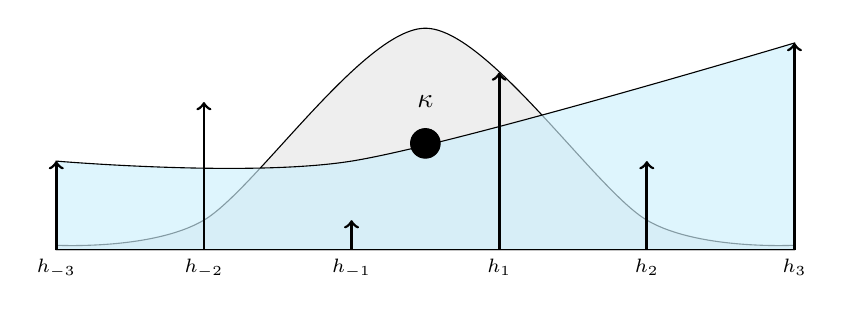
\begin{tikzpicture}[scale=3.75]
	\begin{scope}[fill opacity=0.65]
	\draw [black, fill=gray!20] plot [smooth ] coordinates {(0.25,0.015)(0.75,0.1)(1.50,0.75)(2.25,0.1)(2.75,0.015)} -- (2.75,0) -- (0.25,0) -- cycle;
	
	\draw [black, fill=cyan!20] plot [smooth ] coordinates {(0.25,0.3)(1.25,0.3)(2.75,0.7)} -- (2.75,0) -- (0.25,0) -- cycle;
	\end{scope}
	\draw [fill] (1.5,0.36) circle [radius=0.05];
	\node [above ] at (1.5,0.45) {$\kappa$};
	\draw [arrows=->,line width=1.0] (0.25,0) -- (0.25,0.3);\node [below] at (0.25,0) {\scriptsize $h_{-3}$};
	\draw [arrows=->,line width=1.0] (0.75,0) -- (0.75,0.5);\node [below] at (0.75,0) {\scriptsize $h_{-2}$};
	\draw [arrows=->,line width=1.0] (1.25,0) -- (1.25,0.1);\node [below] at (1.25,0) {\scriptsize $h_{-1}$};
	\draw [arrows=->,line width=1.0] (1.75,0) -- (1.75,0.6);\node [below] at (1.75,0) {\scriptsize $h_{1}$};
	\draw [arrows=->,line width=1.0] (2.25,0) -- (2.25,0.3);\node [below] at (2.25,0) {\scriptsize $h_{2}$};
	\draw [arrows=->,line width=1.0] (2.75,0) -- (2.75,0.7);\node [below] at (2.75,0) {\scriptsize $h_{3}$};
	\end{tikzpicture}
	\caption{Applying a Gaussian filtering kernal to the previous $2^{nd}$ order method allows for an adjustment of scale of the fit.}
	\label{fig:Ghts} 
\end{figure}
In the $5^{th}$ order method, curvature is evaluated at the center of the stencil. However, a more reasonable curvature can be obtained by computing an average curvature over the stencil. This is done by filtering Eqn.~\ref{eqn:poly} with a Gaussian distribution as $\kappa = \int_{-3}^{3} G(\zeta) \kappa(\zeta) d\zeta$. This smooths the polynomial and allows for a more realistic estimation of the curvature. Averaging is achieved using a convolution with a weighting kernel. Transition to $\zeta$ space simplifies this scheme and is defined as $\zeta = \frac{2}{\Delta x}(x-x_i)$. This scheme requires only one floating variable ($\sigma$) as $G(\zeta) = \frac{1}{\sqrt{2 \pi \sigma^2}}e^\frac{- \zeta^2}{2\sigma^2}$. Varying this parameter modifies the scale and filtering kernel of the scheme, allowing optimal operating parameters to be determined. Here, scale refers to the size of the computational stencil with which the curvature is computed as previously described by Owkes et al.~\cite{Owkes2018}. This scheme provided results which were better than previous iterations and significantly more accurate than the standard height function method. However, this model also provided undesirable results at later time steps when simulating an oscillating droplet.     
%\begin{equation}
%\kappa = \int_{-3}^{3} G(\zeta) \kappa(\zeta) d\zeta
%\label{eqn:filt}
%\end{equation} 
%\begin{equation}
%G(\zeta) = \frac{1}{\sqrt{2 \pi \sigma^2}}e^\frac{- \zeta^2}{2\sigma^2}
%\label{eqn:G}
%\end{equation} 

\section{Fine Grid Velocities}
With all  implementations of the fine grid height function we found the remaining existence of interfacial perturbations. While the fine grid height function method does provide a more accurate representation of curvature, it does not reduce or remove these perturbations which are nonphysical and lead to the eventual failure of the simulation. It became clear that actively reducing these discontinuities could provide the interface smoothness necessary for a successful fine grid height function incorporation. To reduce the influence of these perturbations we chose to implement an additional velocity which existed only on the fine grid. The motivation for this can be seen in Figure~\ref{fig:fgvel}, where a discontinuity exists on the fine grid. Our current coarse grid velocity field is unaware of the discontinuity and is thereby, unable to correct this perturbation. However, by incorporating a velocity field on the same scale as the discontinuity, we are able to actively reduce the interfacial perturbation. The following sections will describe this fine grid velocity correction in two parts: fine grid velocity calculation and velocity flux incorporation.                          
\begin{figure}[htbp]
	\centering
	\begin{subfigure}{.3\textwidth}
		\centering
		\includegraphics[width=1.0\linewidth]{figs/fgvel1.png}
		\caption{An interface where a fine grid discontinuity is present.}
		\label{fig:fgVel1}
	\end{subfigure}%
	\hfill
	\begin{subfigure}{0.3\textwidth}
		\centering
		\includegraphics[width=1.0\linewidth]{figs/fgvel2.png}
		\caption{The coarse grid velocity field is unaware of the fine grid perturbation.}
		\label{fig:fgVel2}
	\end{subfigure}
		\hfill
	\begin{subfigure}{0.3\textwidth}
		\centering
		\includegraphics[width=1.0\linewidth]{figs/fgvel3.png}
		\caption{A fine grid velocity correction provides a reaction to the discontinuity.}
		\label{fig:fgVel3}
	\end{subfigure}
	\caption{Motivation for fine grid velocity correction.}
	\label{fig:fgvel}
\end{figure}

\subsection{Implementation of Fine Grid Velocities}
Initial attempts to include a fine grid velocity started by considering a coarse grid cell. Because of the use of a Rudman dual grid, the VOF calculation occurs on the fine grid. The PLIC which represents the interface is also calculated on the fine grid. The discontinuities between PLIC's are what create the parasitic interfacial perturbations which have been discussed. An example of this can be seen in Figure~\ref{fig:PLICS}.
\begin{figure}[htbp]
	\begin{minipage}{0.45\textwidth}
		\centering
%		\includegraphics[width=0.5\linewidth]{figs/PLICS.png}
		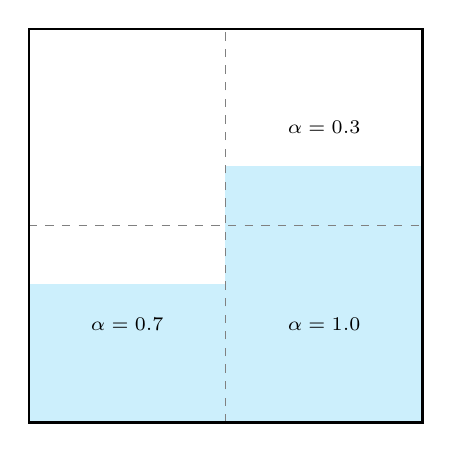
\begin{tikzpicture}[scale=2.5]
		% Mesh
			\draw [cyan!20 ,fill=cyan!20] (0.0,0.0) rectangle (1.0,0.7) ;
			\draw [cyan!20 ,fill=cyan!20] (1.0,0.0) rectangle (2.0,1.3) ;
			\draw [dashed,step=1.0, help lines] (0 ,0) grid (2,2);
			\draw [thick,step=1.0] (0.0 , 0.0) rectangle (2.0,2.0); 
			
			\node at (0.5,0.5) {\scriptsize $\alpha = 0.7$};
			\node at (1.5,0.5) {\scriptsize $\alpha = 1.0$};
			\node at (1.5,1.5) {\scriptsize $\alpha = 0.3$};
			
		\end{tikzpicture}
		\caption{Discontinuities at regions where PLICS join are the source of interface perturbations.}
		\label{fig:PLICS}
	\end{minipage}%
	\hfill
	\begin{minipage}{0.45\textwidth}
	\centering
	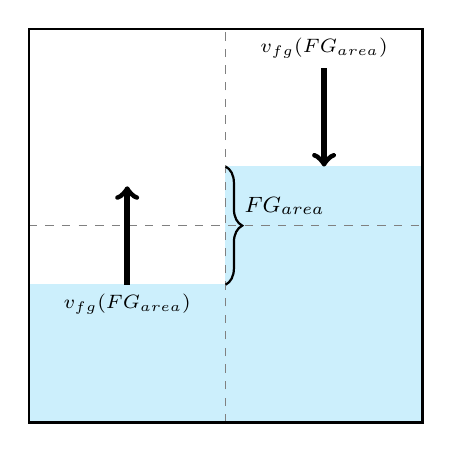
\begin{tikzpicture}[scale=2.5]
	% Mesh
	\draw [cyan!20 ,fill=cyan!20] (0.0,0.0) rectangle (1.0,0.7) ;
	\draw [cyan!20 ,fill=cyan!20] (1.0,0.0) rectangle (2.0,1.3) ;
	\draw [dashed,step=1.0, help lines] (0 ,0) grid (2,2);
	\draw [thick,step=1.0] (0.0 , 0.0) rectangle (2.0,2.0); 
	\draw [thick, decorate,decoration={brace,amplitude=6pt,mirror},xshift=0pt,yshift=0pt](1,0.7) -- (1,1.3) node [black,midway,xshift=0.75cm, yshift=0.25cm] {\footnotesize $FG_{area}$};
	\draw [arrows=->,line width=2.0] (0.5,0.7) -- (0.5,1.2); \node [below ] at (0.5,0.7) {\scriptsize $\bm{v}_{\text{fg}}(FG_{area})$};
	\draw [arrows=->,line width=2.0] (1.5,1.8) -- (1.5,1.3); \node [above ] at (1.5,1.8) {\scriptsize $\bm{v}_{\text{fg}}(FG_{area})$};
	\end{tikzpicture}
	\caption{Discontinuities provide an area with which to scale a fine grid velocity.}
	\label{fig:cor}
	\end{minipage}
\end{figure}
Using a correction velocity which is based on the area of this discontinuity as in Figure~\ref{fig:cor} allows for a proportional correction that is only present where discontinuities exist. This method seemed promising initially by collapsing very simple geometric discontinuities such as those seen in Figure~\ref{fig:cor} but, could not provide adequate solutions for more complex fields such as an oscillating droplet simulation. 

In trying to develop a more robust approach to the area based velocity method, an approach developed by Herrmann was discovered and seemed as though it may provide a  solution~\cite{Herrmann2013}. This method utilizes a spring-damper analogy to approximate interface motion and is derived  originally from the Taylor analogy breakup model (TAB) of O'Rouke and Amsden~\cite{TAB}. The partial differential equation describing the fine grid velocity, $\bm{u}_{\text{fg}},$ proposed by Herrmann  is 

\begin{equation}
\frac{\partial \bm{u}_{\text{fg}}}{\partial t} +
(\bar{\bm{u}}+\bm{u}_{\text{fg}}) \cdot \nabla \bm{u}_{\text{fg}} =
c_{\sigma}\frac{\sigma}{\rho}\bar{\kappa}(\kappa_{\text{fg}}-\bar{\kappa})- 
c_{\mu}\frac{\mu}{\rho L^2}\bm{u}_{\text{fg}}
\label{eqn:HermEq}
\end{equation}
where, $\bar{\bm{u}}$ is the resolved velocity,
$\bm{u}_{\text{fg}}$ is the fine grid velocity,
$\sigma$ is the surface tension coefficient,
$\rho$ is density, 
$\bar{\kappa}$ is the resolved curvature,
$\kappa_{\text{fg}}$ is the fine grid curvature,
$\mu$ is the dynamic viscosity,
$L$ is a modeling length scale and
$C_\sigma$ and
$C_\mu$ are surface tension and viscous scaling coefficients, respectively~\cite{Herrmann2013}. 
The left side of the equation includes a velocity time rate of change as well as a convective term, while the right side includes the surface tension term which acts as a spring force and the viscous term which is analogous to a damping force. By this analogy, system behavior can be moderated by scaling the value on the surface tension or viscous coefficients. One important feature of this method is that it incorporates a difference of coarse grid curvature ($\bar{\kappa}$) and fine grid curvature ($\kappa_{\text{fg}}$). This relation draws a link between the two scales and allows for a coupling of the fine grid and coarse grid methods. While there are several ways to approximate the difference in curvature, we chose to begin with a simple approximation of the coarse grid curvature and used a standard height function method. The fine grid curvature was computed using a second order height function approximation. The generalized update algorithm for Herrmann's equation can be summarized as 
\begin{enumerate}
	\item Solve for coarse grid curvature, $\kappa$, using Eqn.~\ref{eqn:kap}.
	\item Solve for fine grid curvature , $\kappa_{\text{fg}}$, using one of the methods discussed in the previous fine grid height function section.
	\item Interpolate coarse grid curvature to face.This is achieved by assessing curvature at the neighbors left and right of a cell face. If curvature exists in only one of these cells, we interpolate that curvature to the face. If both cells contain interface, a simple average is used to interpolate the curvature to the face. Otherwise no interpolation to a face is necessary.
	\item Compute the gradient of velocity as in Eqn.~\ref{eqn:grad}.
	\item Compute normal vector using an ELVIRA method of Pilliod Jr. and Puckett~\cite{pilliod}.
	\item Compute interface viscous term as a linear average, $\mu =\frac{ \mu_{\text{liq}} + \mu_{\text{gas}}}{2}$.
	\item Compute interface density term as a linear average, $\rho =\frac{ \rho_{\text{liq}} + \rho_{\text{gas}}}{2}$.
	\item Interpolate accompanying fine grid velocity terms (for $\bm{x}$ direction, $\bm{v}$ \& $\bm{w}$ terms are needed) to the fine grid face to use in the convective term of the update equation.
	\item Update fine grid velocity value at cell face using Eqn.~\ref{eqn:update}
	\item Iterate through time as $\bm{u}_{\text{fg}}^{\text{n+1}}  = \bm{u}_{\text{fg}}^{\text{n}}+ \Delta t \bm{u}_{\text{fg, update}}$
\end{enumerate}
The averaging schemes in steps (7) \& (8) above require further explanation. A smooth velocity field normal to the interface provides ideal transport. However, in our experience, large discontinuities in density and viscosity values did not allow for this. While other, more elegant options may exist, the simple averaging method was used as it provided the most stable solutions for our test cases.  

The update equation using equation~\ref{eqn:HermEq},  can be written as 
\begin{equation}
\bm{u_{\text{fg,update}}}= 
-(\bar{\bm{u}}+\bm{u}_{\text{fg}}) \cdot \nabla \bm{u}_{\text{fg}} 
-c_{\sigma}\frac{\sigma}{\rho}\bar{\kappa}(\kappa_{\text{fg}}-\bar{\kappa})- 
c_{\mu}\frac{\mu}{\rho L^2}\bm{u}_{\text{fg}}
\label{eqn:update}
\end{equation}
with the $\bm{x}-$component discretizing as 
\begin{multline}
{u_{\text{fg,update}}}=
- ( \bar{{u}} + {u_{\text{fg}}} ) \frac{d{u_{\text{fg}}}   } { dx} 
- ( \bar{{v}} + {v_{\text{fg}}}     ) \frac{d{u_{\text{fg}}}   } { dy}
- ( \bar{{w}} + {w_{\text{fg}}}    ) \frac{d{u_{\text{fg}}}   } { dz}  \\
- C_{\sigma}\frac{\sigma}{\rho}\kappa(\kappa_{\text{fg}}-\kappa)\bm{n_{\text{x}}} 
- C_{\mu} \frac{\mu {u_{\text{fg}}}}{\rho L^2}  {u_{\text{fg}}}
\end{multline}
and the gradient is discretized using a central finite difference as  
	\begin{equation}
	\nabla \bm{u}_{\text{fg,x}}  =
	\frac{\bm{u_{\text{fg}  }(\text{s$^{+x}$,i$^{+x}$,j,k}) - \bm{u_{\text{fg}  }(\text{s$^{-x}$,i$^{-x}$,j,k})} }}  {  \Delta x_{\text{fg}  }}.
	\label{eqn:grad}
	\end{equation}
 Note that the $s$ index in Eqn.~\ref{eqn:grad} refers to the fine grid cell currently being accessed and the operator $\text{s$^{+x}$}$ refers to the neighboring subcell in the x-direction. Similarly, the $\text{i$^{+x}$}$ is the $i$ index of the neighboring subcell in the x-direction. Illustration of subcell placement can be seen in Figure~\ref{fig:fgOrient}. Because movement within the fine grid can become tedious, NGA incorporates lookup tables which help to minimize confusion. These lookup tables take advantage of the repetitive sequencing of subcell identifiers to ensure correct referencing of neighboring cells and subcells. If subcell index $1$ is being accessed, the left and right neighbor are both subcell index $2$, what changes is the coarse grid index. These quick reference routines make finite differencing operations less confusing by allowing for directional referencing. 
\begin{figure}[htbp]
	\centering
	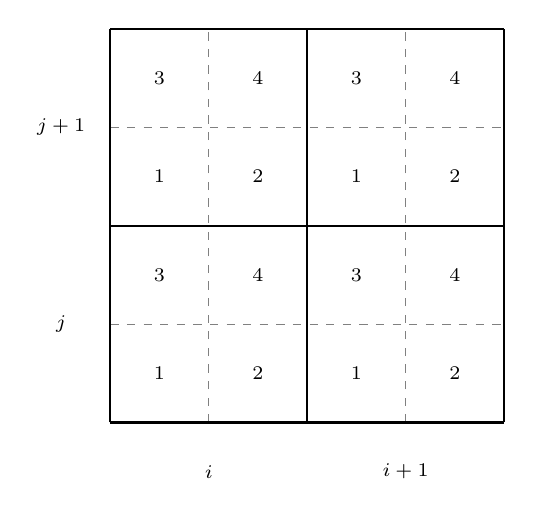
\begin{tikzpicture}[scale=2.5]
	% Mesh
	\draw [dashed,step=0.5, help lines] (0 ,0) grid (2,2);   
	\draw [black, thick, step=1.0] (0 , 0) grid (2,2);
	% subcell identifiers
	\node at (0.25,0.25) {\scriptsize $1$};
	\node at (1.25,0.25) {\scriptsize $1$};
	\node at (0.25,1.25) {\scriptsize $1$};
	\node at (1.25,1.25) {\scriptsize $1$};
	
	\node at (0.75,0.25) {\scriptsize $2$};
	\node at (1.75,0.25) {\scriptsize $2$};
	\node at (0.75,1.25) {\scriptsize $2$};
	\node at (1.75,1.25) {\scriptsize $2$};
	
	\node at (0.25,0.75) {\scriptsize $3$};
	\node at (1.25,0.75) {\scriptsize $3$};
	\node at (0.25,1.75) {\scriptsize $3$};
	\node at (1.25,1.75) {\scriptsize $3$};
	
	\node at (0.75,0.75) {\scriptsize $4$};
	\node at (1.75,0.75) {\scriptsize $4$};
	\node at (0.75,1.75) {\scriptsize $4$};
	\node at (1.75,1.75) {\scriptsize $4$};
	
	% Coarse cell id"s
	\node at (0.5,-0.25) {\scriptsize $i$};
	\node at (1.5,-0.25) {\scriptsize $i+1$};
	\node at (-0.25,0.5) {\scriptsize $j$};
	\node at (-0.25,1.5) {\scriptsize $j+1$};
	
	\end{tikzpicture}
	\caption{Fine grid orientation of subcell indicies. }
	\label{fig:fgOrient}
\end{figure}

\subsection{Modification of Fine Grid Velocity}
Initial results of the fine grid velocity method coupled with height function calculation of curvature suggested a fundamental problem. While explicit curvature calculation remained consistent with previous methods, the oscillating droplet test case again proved difficult. Close inspection of Eq.~\ref{eqn:HermEq} reveals that the equation is not well-poised when the coarse-grid curvature, $\bar{\kappa}$, is zero as the entire spring force goes to zero even if fine-grid interface perturbations exist and $\kappa_{\text{fg}} \neq 0$.  An alternative is to base the source term on the difference between coarse and fine-grid curvatures and add a delta function that restricts the source term to only be non-zero at the interface. This term was chosen as it is also the source term used in the Navier-Stokes equations. The approximation of the Dirac delta function is calculated as the absolute difference in liquid volume fractions between cells divided by the mesh size as
\begin{equation}
\delta = \frac{|\alpha(\text{s,i,j,k}) - \alpha(\text{s$^-$,i$^-$,j,k}) | }{0.5 \Delta x}.
\label{eqn:delta}
\end{equation}
Additionally, a pressure term is added to ensure fine grid velocity remains divergence free, further enforcing momentum conservation. The current pressure method, a simple Poisson equation where 
\begin{equation}
-\nabla P = \frac{\bm{u}^{n+1} - \bm{u}^*}{\Delta t},
\label{eqn:poisson}
\end{equation}does have the disadvantage of being computationally expensive. In his original work, Herrmann has an alternate method for computing a divergence free velocity field which if incorporated, may prove more economical~\cite{Herrmann2013}. However, a Poisson equation is robust and easy to implement. This may be an area worth exploring in future work. With these modifications, the proposed equation to create the fine-grid velocity can be written as
\begin{equation}
\frac{\partial \bm{u}_{\text{fg}}}{\partial t} +
(\bar{\bm{u}}+\bm{u}_{\text{fg}}) \cdot \nabla \bm{u}_{\text{fg}} = 
c_{\sigma}\frac{\sigma}{\rho}\delta(\kappa_{\text{fg}}-\bar{\kappa})- 
c_{\mu}\frac{\mu}{\rho L^2}\bm{u}_{\text{fg}} -
\nabla P_{\text{fg}}
\label{eqn:MyEq}
\end{equation}
along with the continuity equation
\begin{equation}
\nabla\cdot\bm{u}_\text{fg}=0.
\end{equation}
The modified update algorithm is now
\begin{enumerate}
	\item Solve for coarse grid curvature, $\kappa$, using Eqn.~\ref{eqn:kap}.
	\item Solve for fine grid curvature , $\kappa_{\text{fg}}$, again using Eqn.~\ref{eqn:kap} but with the $2^{nd}$ order method as outlined previously.
	\item Interpolate coarse grid curvature to face.This is achieved by assessing curvature at the neighbors left and right of a cell face. If curvature exists in only one of these cells, we interpolate that curvature to the face. If both cells contain interface, a simple average is used to interpolate the curvature to the face. Otherwise no interpolation to a face is necessary.
	\item Compute the gradient of velocity as in Eqn.~\ref{eqn:grad}.
	\item Compute normal vector using an ELVIRA method of Pilliod Jr. and Puckett~\cite{pilliod}.
	\item Compute viscous term as a linear average, $\mu =\frac{ \mu_{\text{liq}} + \mu_{\text{gas}}}{2}$.
	\item Compute density term as a linear average, $\rho =\frac{ \rho_{\text{liq}} + \rho_{\text{gas}}}{2}$.
	\item Interpolate accompanying fine grid velocity terms (for $\bm{x}$ direction, $\bm{v}$ \& $\bm{w}$ terms are needed) to the fine grid face to use in the convective term of the update equation.
	\item Calculate delta function using Eqn.~\ref{eqn:delta}
	\item Predict fine grid velocity value at cell face as 
%	\begin{equation}
%	\bm{u^{\text{fg,update}}}= 
%	-(\bar{\bm{u}}+\bm{u}_{\text{fg}}) \cdot \nabla \bm{u}_{\text{fg}} 
%	-c_{\sigma}\frac{\sigma}{\rho}\delta(\kappa_{\text{fg}}-\bar{\kappa})- 
%	c_{\mu}\frac{\mu}{\rho L^2}\bm{u}_{\text{fg}}
%	\label{eqn:myupdate}
%	\end{equation}
	\begin{equation}
	\bm{u}^{*}= \bm{u}^{\text{n}} - \Delta t(
	(\bar{\bm{u}}+\bm{u}_{\text{fg}}) \cdot \nabla \bm{u}_{\text{fg}} 
	+c_{\sigma}\frac{\sigma}{\rho}\delta(\kappa_{\text{fg}}-\bar{\kappa}) 
	+c_{\mu}\frac{\mu}{\rho L^2}\bm{u}_{\text{fg}})
	\label{eqn:myupdate}
	\end{equation}
	\item Solve pressure Poisson equation using Eqn.~\ref{eqn:poisson}
	\item Correct velocity value using updated pressure field as 
	\begin{equation}
	\bm{u}^{\text{n}+1} = \bm{u}^* - \nabla P \Delta t
	\end{equation}
%	\item Iterate through time as $\bm{u}_{\text{fg}}^{\text{n+1}}  = \bm{u}_{\text{fg}}^{\text{n}}+ \Delta t \bm{u}_{\text{fg, update}}$
\end{enumerate}

Test case results from this iteration again did not represent successful implementation. We began considering the relationship of the difference in curvatures. We considered that the difference in curvatures may introduce an error that is due to the different ways the two curvatures are calculated and not just from the interface perturbations that we were trying to measure. To eliminate this added error a new approach for the coarse grid curvature estimate was necessary. It seemed that there were various ways to approximate the coarse grid curvature $\bar{\kappa}$ but, that our goal was to influence this value with information from the fine grid. One approximation for $\bar{\kappa}$ is that it is made up as an average of the fine grid curvatures. That is, for a single given coarse grid cell, the average of the fine grid curvatures should produce a value close to the coarse grid curvature. We changed the calculation of the coarse grid curvature such that it was an average value of the fine grid curvatures using a simple linear averaging technique as 
\begin{equation}
\bar{\kappa} = \frac{1}{8} \sum_{s} \kappa_{\text{fg}} 
\end{equation} where $s$ denotes the sum over subcells. An advantage of this method was that it tied the fine grid velocity to one curvature, the fine grid curvature. This provided us with more freedom over how to calculate the fine grid curvature value and removed a second dependency (the value of $\bar{\kappa}$) for calculating fine grid velocity in our update equation. This method also allowed for a variation in the scale of the smearing acting over the coarse grid curvature. Initially, the curvature was calculated as the average of the fine grid curvatures within the cell. An advantageous extension of this method  allows for further smearing to include information of surrounding cells by
 \begin{equation}
 \bar{\kappa} = \frac{1}{(2N)^3}\sum_{i=i-N}^{i+N}\sum_{j=j-N}^{j+N} \sum_{k=k-N}^{k+N} \kappa_{\text{fg}} ,
 \end{equation}
 where $N$ is the number of cells over which you want to smear the curvature calculation.
 
  Equation~\ref{eqn:MyEq} is representative of the scheme implemented at the time of this publication.  Additional efforts were taken to  find an optimal parameterization strategy with little success. Figure~\ref{fig:para} shows a parameterization study where $C_{\sigma}$ and $C_{\mu}$ varied from $1e^{-6}$ to $1e^6$ and an oscillating droplet test case was ran. While a portion of the runs seem initially successful looking at Figure~\ref{fig:para2} shows a discrepancy between acceptable values when switching the case to be ran on a finer grid. Tuned parameter values were not found to be consistent across various mesh sizes and no conclusive optimal configuration was found. 
\begin{figure}[htbp]
	\centering
	\begin{tikzpicture}
		\node[anchor=south west,inner sep=0] at (0,0) {\includegraphics[width=1.0\linewidth]{figs/para}};
		\node at  (2.3,0.5) {\scriptsize $1e^{-6}$};
		\node at  (13.4,0.5) {\scriptsize $1e^{6}$};
		\node at  (8.0,-0.25) {$\bm{C_{\sigma}}$};
		\node at  (1.5,1.0) {\scriptsize $1e^{6}$};
		\node at  (1.5,7.0) {\scriptsize $1e^{-6}$};
		\node at  (0.5,4.25) {$\bm{C_{\mu}}$};
	\end{tikzpicture}
	\caption{Parameterization study of an oscillating droplet test case (64x mesh size). Plots show kinetic energy over time as seen in previous studies. The varying parameters are $C_{\sigma}$ and $C_{\mu}$ which vary from $1e^{-6}$ to $1e^6$.}
	\label{fig:para}
\end{figure}
\begin{figure}[htbp]
	\centering
	\begin{tikzpicture}
	\node[anchor=south west,inner sep=0] at (2.0,0.65) {\includegraphics[width=0.76\linewidth]{figs/para2}};
	\node at  (2.3,0.5) {\scriptsize $1e^{-6}$};
	\node at  (13.4,0.5) {\scriptsize $1e^{6}$};
	\node at  (8.0,-0.25) {$\bm{C_{\sigma}}$};
	\node at  (1.5,1.0) {\scriptsize $1e^{6}$};
	\node at  (1.5,7.0) {\scriptsize $1e^{-6}$};
	\node at  (0.5,4.25) {$\bm{C_{\mu}}$};
	\end{tikzpicture}
	\caption{Parameterization study of an oscillating droplet test case (128x mesh size). Plots show kinetic energy over time as seen in previous studies. The varying parameters are $C_{\sigma}$ and $C_{\mu}$ which vary from $1e^{-6}$ to $1e^6$.}
	\label{fig:para2}
\end{figure}


\section*{Fine Grid Velocity Flux  Incorporation} 
Away from the phase interface, NGA uses high-order finite difference operators that conservatively transport mass, momentum, and any other scalars~\cite{NGA2}.  Near the phase interface however, the finite difference operators are inappropriate due to the discontinuous interface region.  To accurately and conservatively transport near the interface, an unsplit geometric semi-Lagrangian flux method is used~\cite{Owkes2017,Owkes2014}. This method relies on signed streaktubes, which contain the region of the domain that moves through a computational cell face during the time step~\cite{Owkes2017}.  The streaktube is represented with a collection of tetrahedra as shown in Figures~\ref{fig:streak} \&~\ref{fig:simp} and computational geometry is used to compute the flux of liquid, mass, momentum, and any scalars~\cite{Owkes2017}. A correction is incorporated which forces a solenoidal condition for the cell. The scheme contains two primary steps. First, a project function creates a flux volume by moving points on the cell face back in time in a Lagrangian sense as seen in Figure~\ref{fig:streak}. To provide a better explanation of this step, we can assume  that for a position $\bm{x}$, we know that 
\begin{equation}
\frac{d \bm{x}}{d t} = \bm{u}.
\end{equation} 
This can be approximated as 
\begin{equation}
\bm{x}^n = \bm{x}^{n+1} - \Delta t \bm{u}^{n+1}.
\end{equation} The volume which was projected is then broken up into simplicies. These simplicies are first cut by the grid cell, then by PLIC. This continues until all simplicies contain only one phase as described in the previous section and shown in Figure~\ref{fig:simp}. Simplicies (tetrahedra in 3D)  constructed of only liquid ensure consistent mass and momentum transport. 

The addition of a fine grid velocity requires that the additional velocity be incorporated into the flux, this is achieved by adjusting the streaktube scheme. However, several different options exist for doing so. Initially, we incorporated the fine grid velocity directly into the project function. The project function uses information about the velocity field to determine the amount of flux through a cell face. While this method works well across coarse cell faces, it does not always work between subcell faces. As illustrated by Figure~\ref{fig:net0}, when the net velocity being fluxed over subcells within a coarse cell is zero, the project function would assume there was no additional flux to be accounted for. In the case of Figure~\ref{fig:net0}, the value of interest (the fine grid velocity correction) must be interpolated to the cell center for use in the project function. It is clear that for this scenario the two vertical velocities of equal and opposite magnitude would exactly cancel out. This results in no fine grid velocity correction being incorporated into the project function. This does not provide a consistent scheme as the fine grid divergence would not be equal to zero globally as required. 
\begin{figure}[htbp]
	\centering
	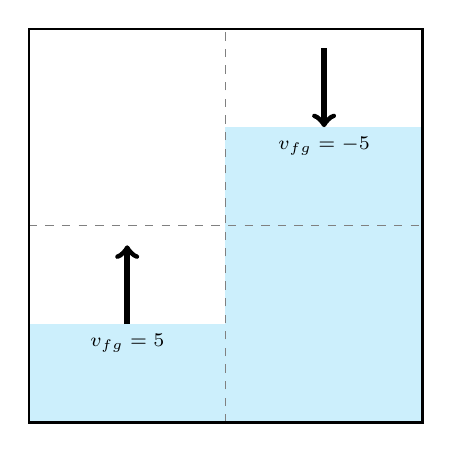
\begin{tikzpicture}[scale=2.5]
	% Mesh
	\draw [cyan!20 ,fill=cyan!20] (0.0,0.0) rectangle (1.0,0.5) ;
	\draw [cyan!20 ,fill=cyan!20] (1.0,0.0) rectangle (2.0,1.5) ;
	\draw [dashed,step=1.0, help lines] (0 ,0) grid (2,2);
	\draw [thick,step=1.0] (0.0 , 0.0) rectangle (2.0,2.0); 
	\draw [arrows=->,line width=2.0] (0.5,0.5) -- (0.5,0.9); \node [below ] at (0.5,0.5) {\scriptsize $\bm{v}_{\text{fg}} =  5$};
	\draw [arrows=->,line width=2.0] (1.5,1.9) -- (1.5,1.5); \node [below ] at (1.5,1.5) {\scriptsize $\bm{v}_{\text{fg}} = -5$};
	\end{tikzpicture}
	\caption{Where net velocity fluxing within a coarse cell is zero, the project function does not incorporate the necessary flux values.}
	\label{fig:net0}
\end{figure}
Seeing this error, we moved to manually adjusting the streaktubes. So, after the project function projects vertices back in time to construct the streaktubes, streaktubes are partitioned into simplices. We adjusted the simplicies such that the total volume of the streaktube included the fine grid velocity values. Originally the total streaktube volume could be calculated as 
\begin{equation}
	V_{st} = \bm{u} A_{CS}\Delta t .
\end{equation}
Adding the fine-grid velocity correction is done by modifying the additional flux due to the fine-grid velocities so that the volume becomes
\begin{equation}
V_{st} = (\bm{u}_{\text{cg}}  + \bm{u}_{\text{fg}} )A_{CS}\Delta t .
\end{equation}  This addition provides an explicit numerical representation of the fine grid velocity correction and maintains conservation laws. 

\subsection{Results of Current Implementation}
As previously stated, the incorporation of the fine grid height function, fine grid velocity, and flux incorporation all happened simultaneously. However, a description of all methodologies have now been provided. The current implementation uses a second order height function method for both the coarse gird and fine grid curvature estimation. Fine grid velocity correction is achieved using Eqn.~\ref{eqn:myupdate} and the pressure correction method described previously. Velocity incorporation into the cell flux uses a combination method of streaktube modification and additional simplicies to fully capture the dynamics caused by the fine grid velocity. With the most recent iteration of all three schemes integrated into the fine grid method, the baseline test cases were once again evaluated. Results are shown in Figures~\ref{fig:fgVelCurv}~\&~\ref{fig:fgVelKE} and show considerable improvement from the standard height function method. However, test cases still resulted in nonphysical dynamics when moving to more complex geometries such as 3D flow fields. All test cases examined which include three dimensional geometry resulted in errors which eventually caused simulation failure. Because of this continued failure, it seemed appropriate to reevaluate the validity of the original methodology and take a deeper look into the mechanisms which were the cause of these deficiencies.
\begin{figure}[htbp]
	\centering
	\begin{subfigure}{.45\textwidth}
		\centering
		\includegraphics[width=1.0\linewidth]{figs/curvCalc.png}
		\caption{Calculation of an exact VOF field by the current implementation of the fine grid curvature scheme.}
		\label{fig:fgVelCurv}
	\end{subfigure}%
	\hfill
	\begin{subfigure}{0.45\textwidth}
		\centering
		\includegraphics[width=1.0\linewidth]{figs/current_KEplot.png}
		\caption{Kinetic energy plotted over time for an oscillating droplet test case. Current implementation (Solid) ACES method (Dashed)}
		\label{fig:fgVelKE}
	\end{subfigure}
\caption{Results from current implementation.}
\end{figure}

\section{Simplified Test Cases}
With each of the schemes previously discussed, the method of evaluation consisted of an explicit curvature calculation of an exact VOF field followed by an oscillating droplet test case. Consistently, the exact curvature estimation was successful and the oscillating droplet problematic. The transition between the test cases began to seem like too great of a jump in complexity to have an intimate understanding of the progression of errors occurring. To gain a deeper understanding of the source of failure, it seemed necessary to have more simplified test cases with which to study the method. To this end, four simplified test cases were developed which we hoped would expose the limitations of the schemes.

\subsection{Sine Wave Test Case}
A sinusoidal interface was constructed as seen in Figure~\ref{fig:sine}. The test case was created specifically to test several key aspects of the method. First, by modifying the geometry of the sinusoid its possible to test face fluxes by watching the simulation progress through the coarse cell as well as the fine grid cells. Having a consistent transition from coarse grid faces to fine grid faces ensured that fluxes were being treated consistently across the domain. Secondly, because the interface is highly symmetric, variation in velocity and curvature values across the domain helps to highlight deficiencies in boundary conditions as well as inter-cell transport schemes. The goal of this test case is for the fine grid scheme to force a collapse of the interface so that a final curvature of zero is achieved.  
\begin{figure}[htbp]
	\centering
	\includegraphics[width=0.5\textwidth]{figs/sine}
	\caption{A simplified geometry test case is presented with a sinusoidal interface.}
	\label{fig:sine}
\end{figure}

\subsection{Interfacial Protrusion Test Case}
The test cases shown in Figures~\ref{fig:0},~\ref{fig:90},~\&~\ref{fig:45} are all of a simple linear interface at various orientations. At the center of each domain, a protrusion was placed on the interface. The aim of this test case was to recreate specific, isolated, scenarios to see if the fine grid method could accomplish collapsing the interface to a line and obtain a zero curvature across the domain. The protrusion on each interface was built to be approximately one cell width in both height and width.  

\begin{figure}[htbp]
	\centering
	\begin{subfigure}{0.3\textwidth}
		\fbox{\includegraphics[width=0.95\linewidth]{figs/0}}
		\caption{A simplified geometry test case is presented with a horizontal interface that includes a protrusion of approximately one cell width.}
		\label{fig:0}
	\end{subfigure}%
\hfill
	\begin{subfigure}{0.3\textwidth}
		\fbox{\includegraphics[width=0.95\linewidth]{figs/90}}
		\caption{A simplified geometry test case is presented with a vertical interface that includes a protrusion of approximately one cell width.}
		\label{fig:90}
	\end{subfigure}
\hfill
	\begin{subfigure}{0.3\textwidth}
		\fbox{\includegraphics[width=0.95\linewidth]{figs/45}}
		\caption{A simplified geometry test case is presented with a diagonal interface that includes a protrusion of approximately one cell width.}
		\label{fig:45}
	\end{subfigure}
\caption{Interfacial perturbation test cases.}
\end{figure}

\subsection{Results}
\begin{figure}[htbp]
	\centering
	\fbox{\includegraphics[width=0.5\linewidth]{figs/45new.png}}
	\caption{Result of $45^{\circ}$ test case showing nonphysical dynamics at simulation completion.}
	\label{fig:45new}
\end{figure}
For each of the above test cases, with the exception of the $45^{\circ}$ test case, the method was successful in collapsing the interface to a line. Instead, the $45^{\circ}$ case final state can be see in Figure~\ref{fig:45new}.  This was an interesting discovery and seemed to coincide with results seen in failing oscillating droplet test cases. During the oscillating droplet test, often nonphysical geometries would begin to appear at each of the quadrant regions of the droplet as shown in Figure~\ref{fig:45s}. This finding exposed a key limitation of the model. Well defined heights are not present in this case and cause problems for the height function method. When heights are not well defined, the approximation of derivatives is not accurate and results in nonphysical geometries. The problematic region is highlighted in Figure~\ref{fig:probhts2}. Here, we can see that using heights or widths can result in a region of ill-defined heights. The only way to avoid this complication is with mesh refinement. However, instead of indicating an ill-defined test case, this suggests a general shortcoming of height functions.
\begin{figure}[htbp]
	\centering
	\includegraphics[width=0.4\linewidth]{figs/bad.png}
	\caption{Result displaying nonphysical structures typically found in failing oscillating droplet simulations. Often, structures would grow from the four quadrant regions where well defined heights are hardest to obtain.}
	\label{fig:45s}
\end{figure}
\begin{figure}[htbp]
	\centering
\includegraphics[width=0.5\linewidth]{figs/probhts.png}
	\caption{For the diagonal protrusion test case it is evident that the height function is unable to create the necessary well defined heights that are required for an accurate curvature estimation when a protrusion is on the order of a coarse grid cell.}
	\label{fig:probhts2}
\end{figure}








